\chapter{Implementation - "Building the solution"}


\section{Introduction}

This chapter is a walkthrough of the steps which describe the construction of the application.

\section{Terminal}

\subsection{Command Line Instructions}

As this application was centred towards security and being secure as the data it would hold would need to be kept safe. Therefore it made sense to focus on a good login with authentication and authorisation. To start working with Symfony, one needs to setup the Symfony enviroment through an installation process before Symfony applications can be created. Instructions for this can be found on the SensioLabs Symfony website. Navigating to the Documentation page. In there can be found Chapter 1 which has the Setup instructions under the Get Started dropdown menu. They explain the different ways for installing and setting up the Symfony framework for both Mac OS and Windows. Along with some\newline troubleshooting ideas if there are any problems with the installation. This application was built on a Mac OS so the instructions would vary slightly due to the command line instructions used. Using the installer made it easy to create this application with Symfony and only needed to be done once as it was installed globally on the machine.

\begin{figure}[htbp]
   \centering
   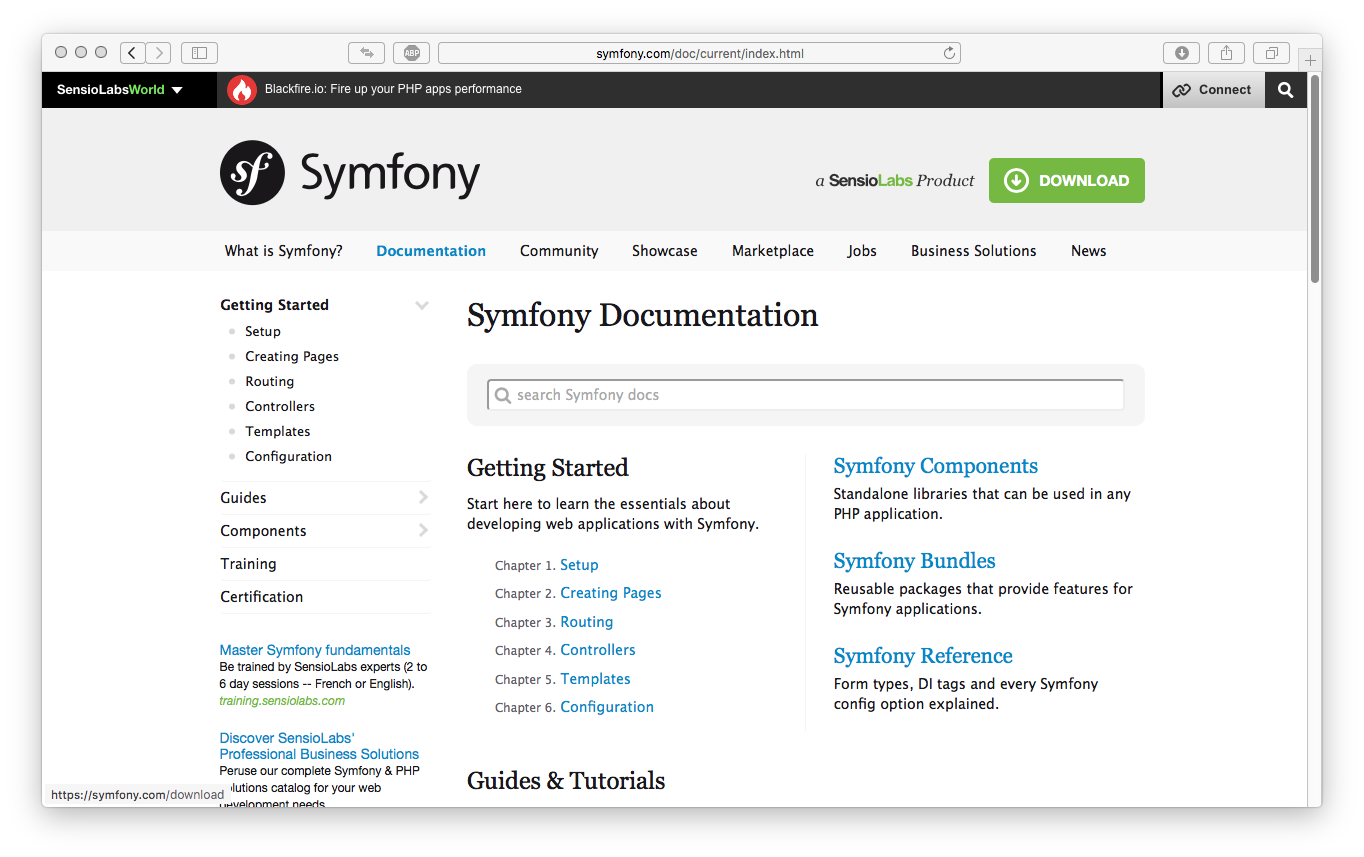
\includegraphics[width=400pt]{figures/symfony_documentation.png} % requires the graphicx package
   \caption{Symfony Documentation}
   \label{fig:Symfony Documentation}
\end{figure}

\begin{figure}[htbp]
   \centering
   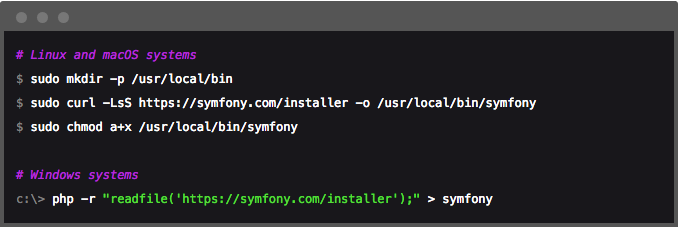
\includegraphics[width=400pt]{figures/symfony_installation.png} % requires the graphicx package
   \caption{Symfony Installation Setup}
   \label{fig:Symfony Installation Setup}
\end{figure}

With this completed moving into the directory or environment that the application will live which was the desktop. A final command in the terminal window was issued. This time starting with symfony new and by giving a project a name of choice thereafter. In this case the name COMPH4021-Project was used. The project was based on the current version of Symfony which is version 3.2.8. However, other versions can be specified after the project name in the terminal window. Once this part was completed. All required components were downloaded into a project folder with the name of which was given. The components are a set of files and directories which form the web application which use the Symfony libraries. The installer also carries out a check to make sure all requirements are met. If requirements are not all met a list is generated which provides the changes that are needed. In this case no changes needed to be made.

\begin{figure}[htbp]
   \centering
   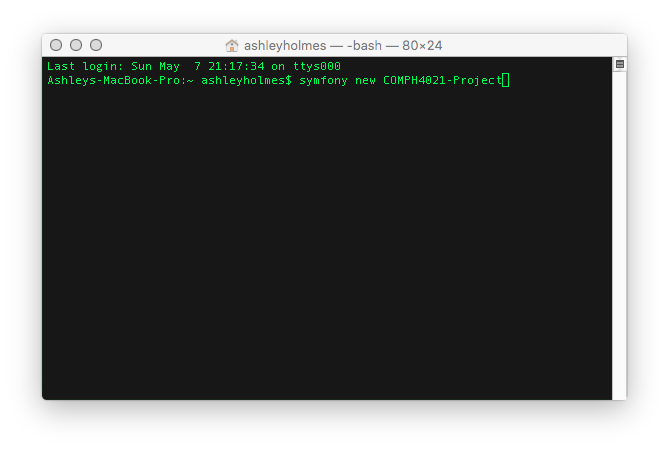
\includegraphics[width=400pt]{figures/new_application.png} % requires the graphicx package
   \caption{Symfony Application Setup}
   \label{fig:Symfony Application Setup}
\end{figure}

The below figure \ref{fig:Terminal Window Top} displays the command issued to download the project folder and following that in figure \ref{fig:Terminal Window Bottom} one can see that the project is being prepared and where it will be stored. In this case it was stored in /Users/ashleyholmes/Desktop/COMPH4021-Project.

\begin{figure}[htbp]
   \centering
   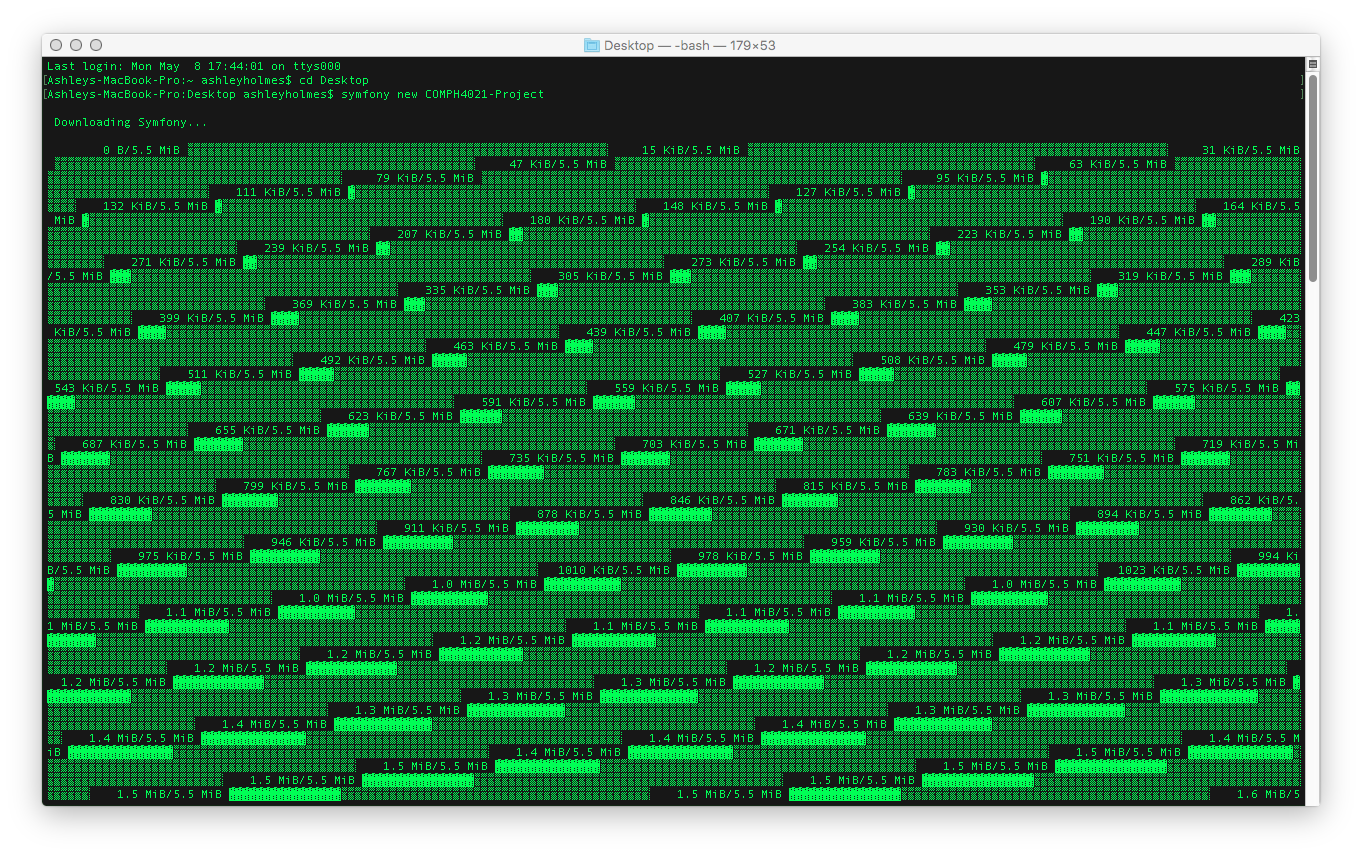
\includegraphics[width=400pt]{figures/terminal_window_top.png} % requires the graphicx package
   \caption{Terminal Window Top}
   \label{fig:Terminal Window Top}
\end{figure}

\begin{figure}[htbp]
   \centering
   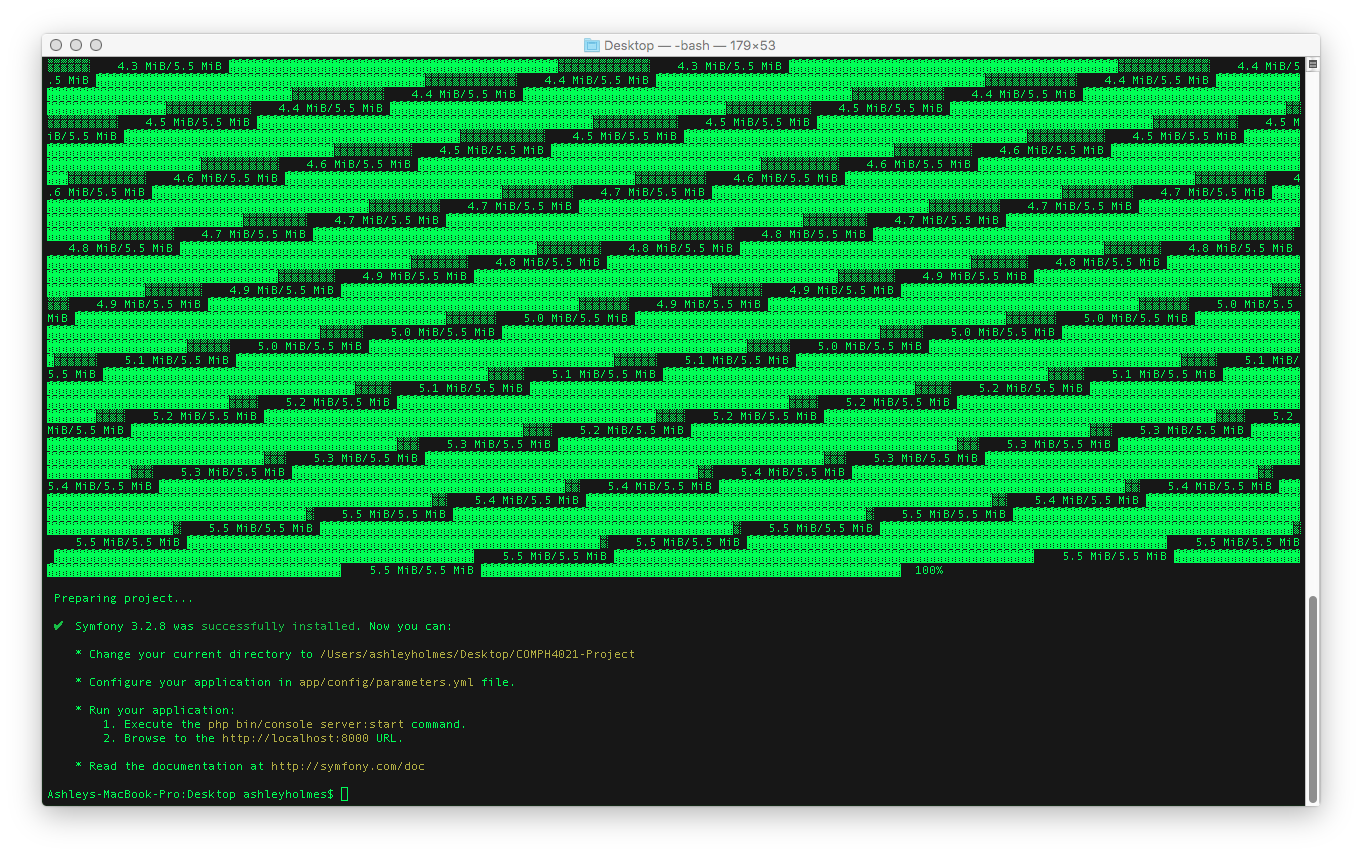
\includegraphics[width=400pt]{figures/terminal_window_bottom.png} % requires the graphicx package
   \caption{Terminal Window Bottom}
   \label{fig:Terminal Window Bottom}
\end{figure}

\begin{figure}[htbp]
   \centering
   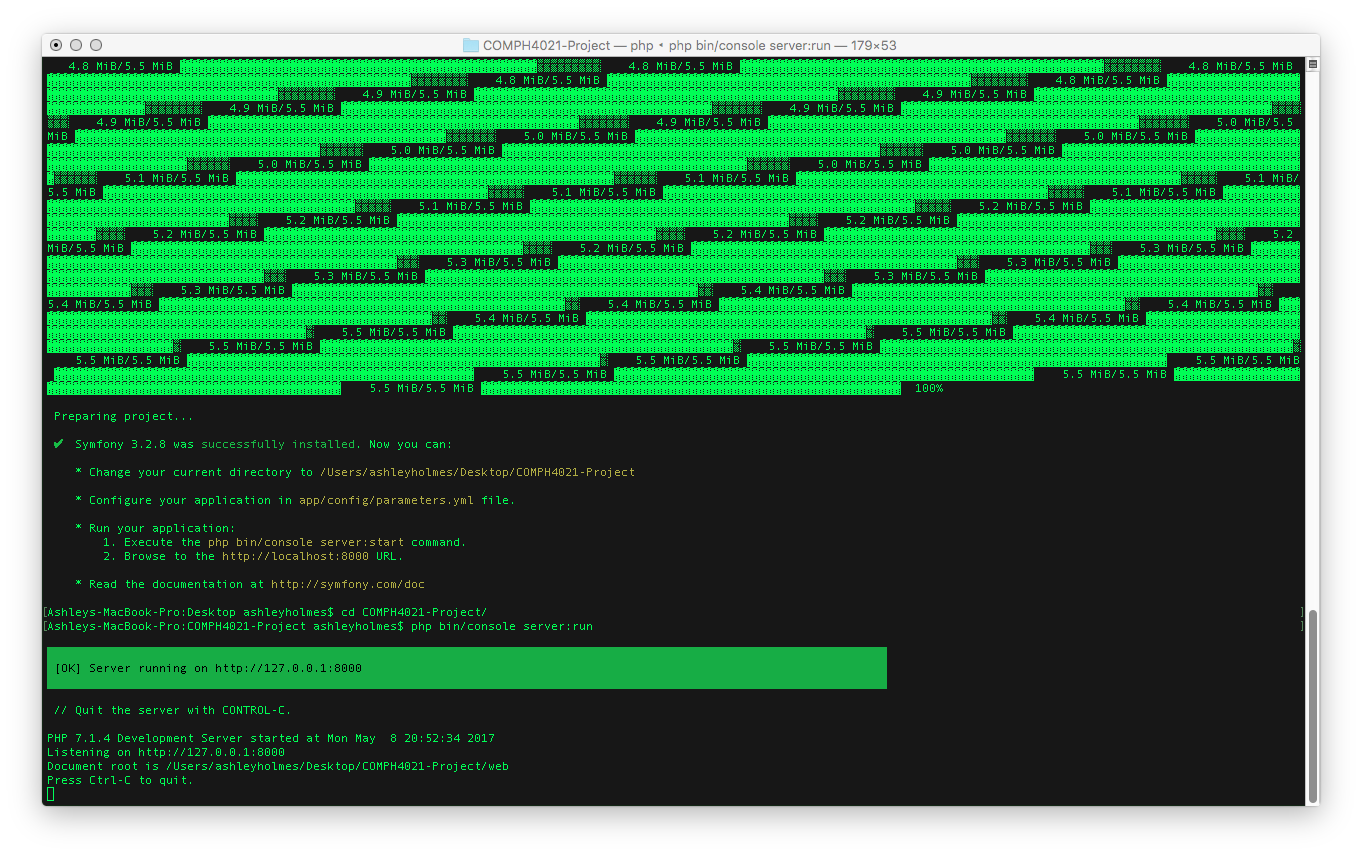
\includegraphics[width=400pt]{figures/php_server_run.png} % requires the graphicx package
   \caption{Php Server Run}
   \label{fig:Php Server Run}
\end{figure}

\begin{figure}[htbp]
   \centering
   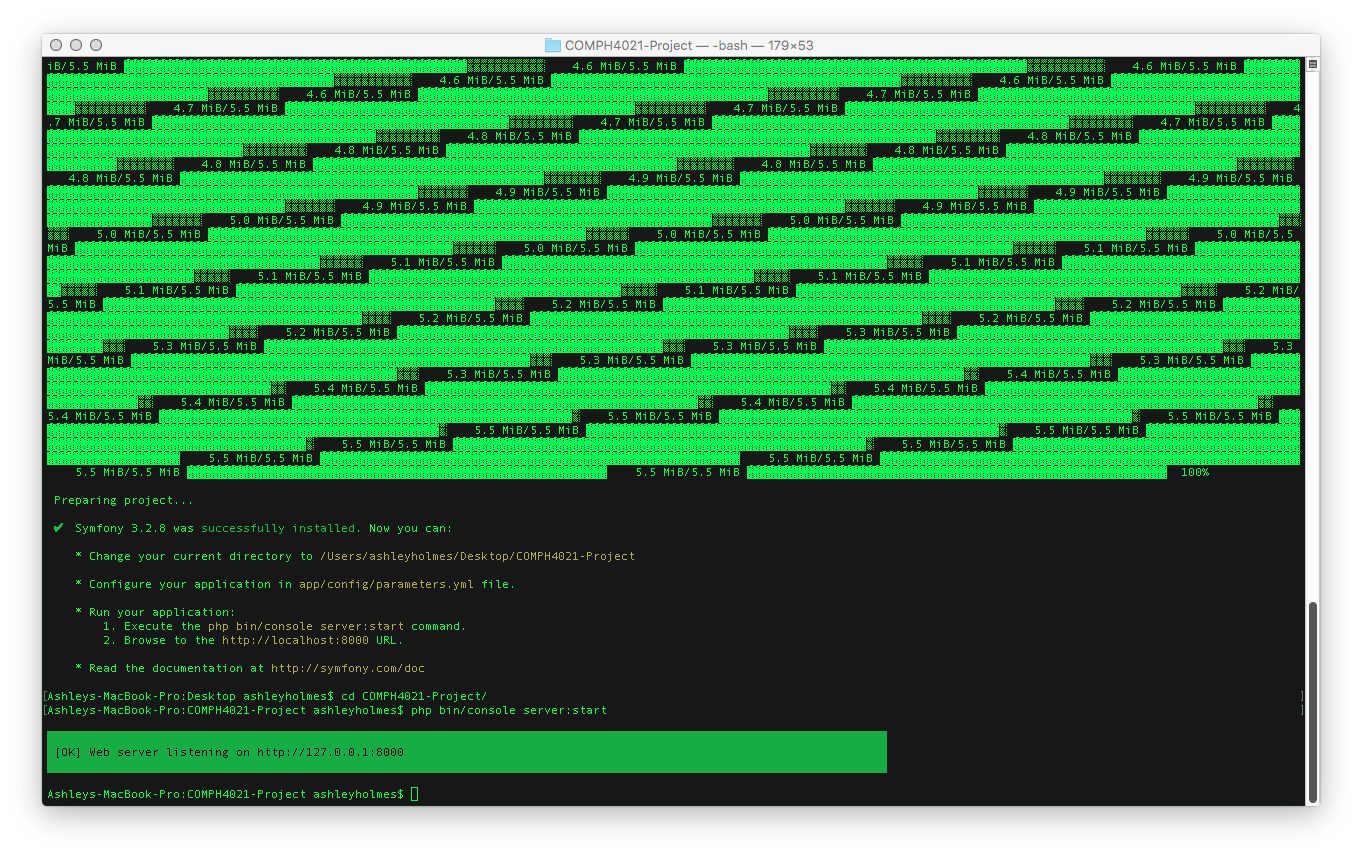
\includegraphics[width=400pt]{figures/php_server_start.png} % requires the graphicx package
   \caption{Php Server Start}
   \label{fig:Php Server Start}
\end{figure}

The next step would be to change directory into the COMPH4021-Project directory as this is where the built in Php server needs to be run from. NGINX and Apache may be used as alternatives however, since the Php server is built in. It makes development much easier. Executing the following command php bin/console server:run starts the server. However, once issuing this command the open terminal window would now need to remain out of use while the server is running. One can use a separate terminal window or open a new tab to issue any addition commands which are needed or make use of the PhpStorm terminal window. To run other processes in the background, issuing a php bin/console server:start will make it possible to execute commands in the same window which was done here. The difference can be seen in figure \ref{fig:Php Server Run} and figure \ref{fig:Php Server Start}.

\section{Browser}

\subsection{Deploying the Application}

\begin{figure}[htbp]
   \centering
   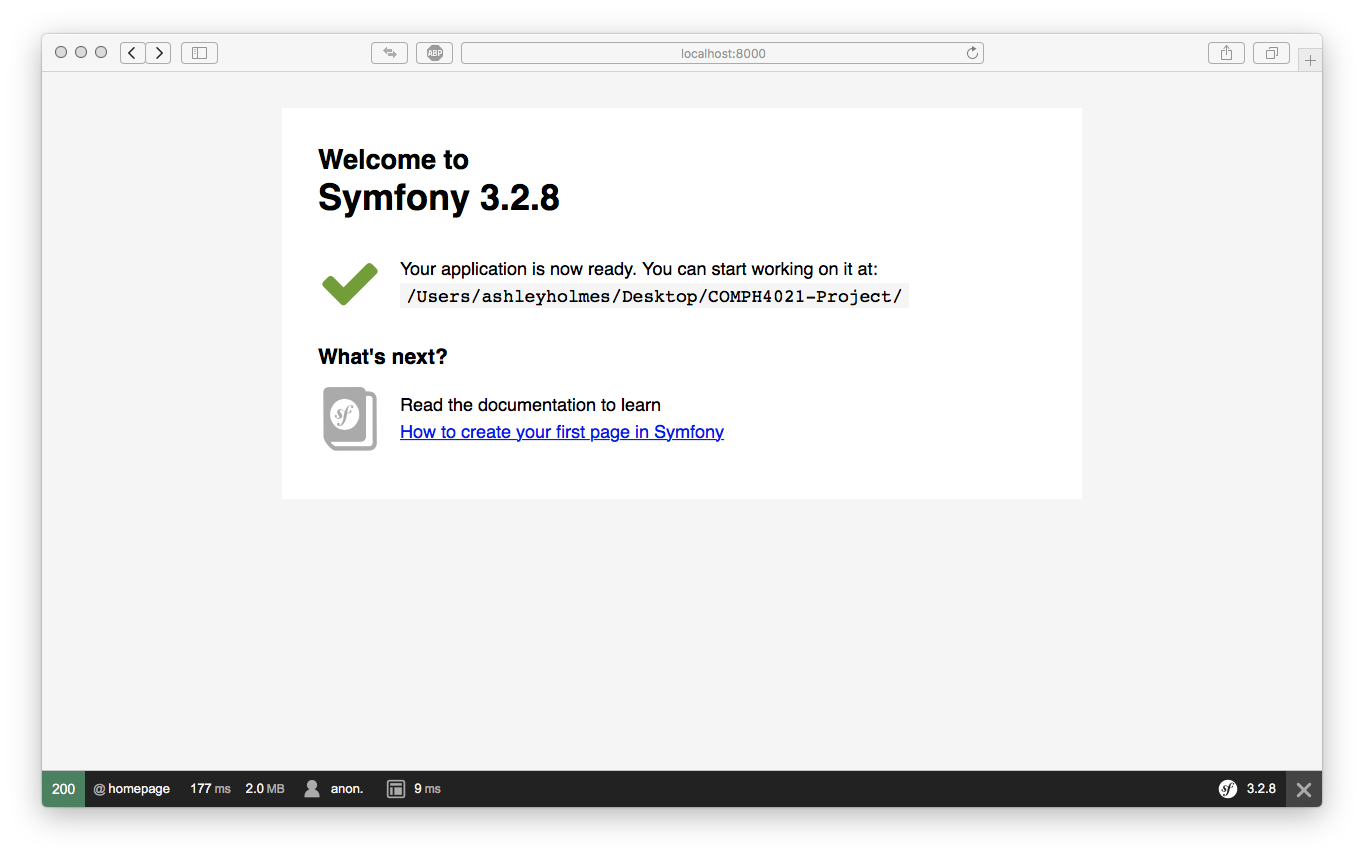
\includegraphics[width=400pt]{figures/symfony_browser.png} % requires the graphicx package
   \caption{Symfony Browser}
   \label{fig:Symfony Browser}
\end{figure}

\begin{figure}[htbp]
   \centering
   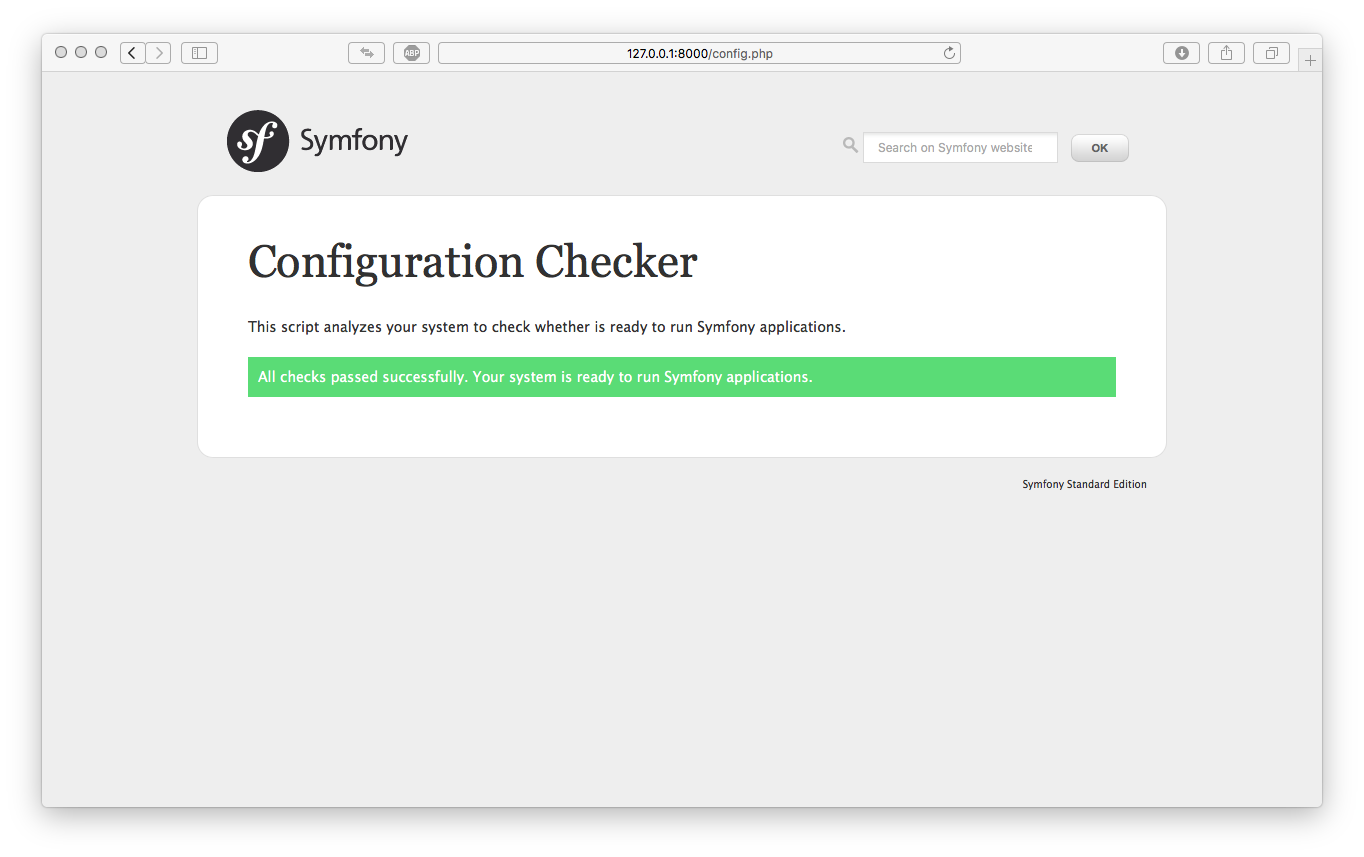
\includegraphics[width=400pt]{figures/configuration_checker.png} % requires the graphicx package
   \caption{Configuration Checker}
   \label{fig:Configuration Checker}
\end{figure}

\begin{figure}[htbp]
   \centering
   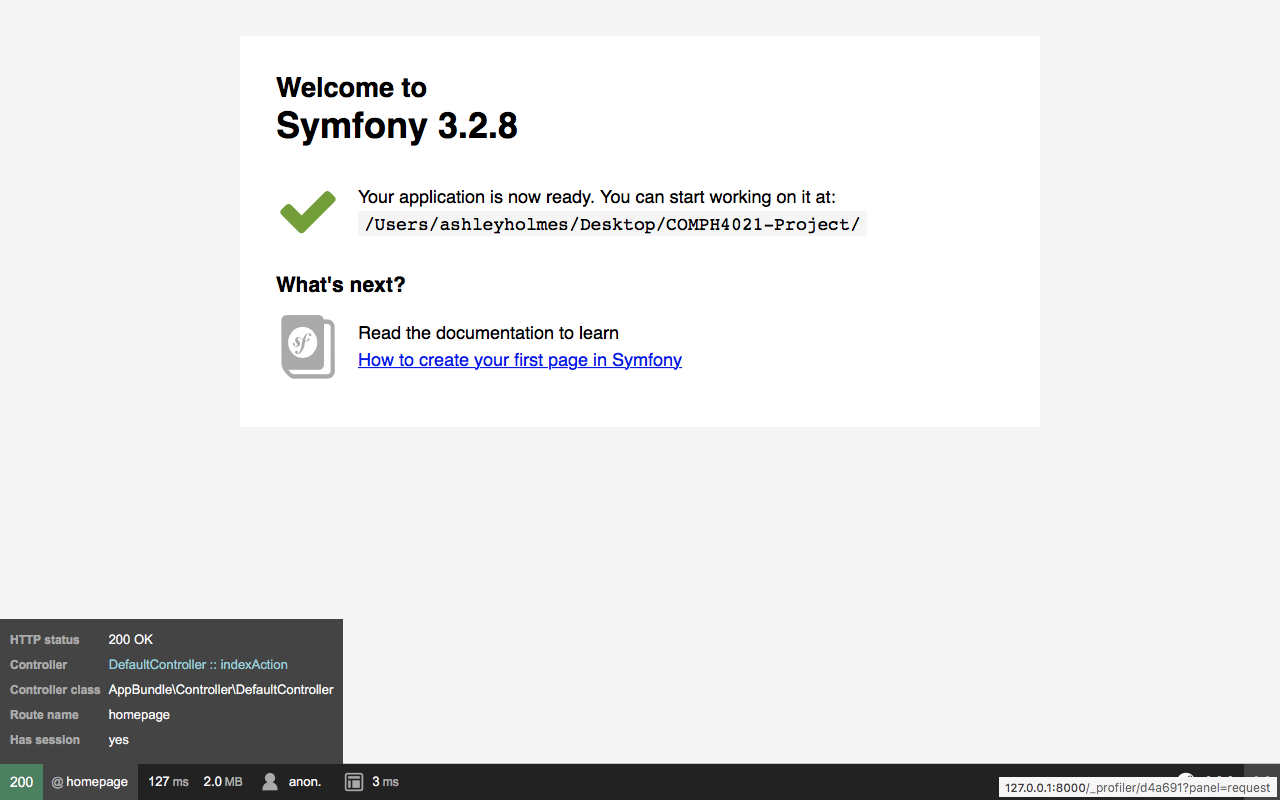
\includegraphics[width=400pt]{figures/webdebug_1.png}
   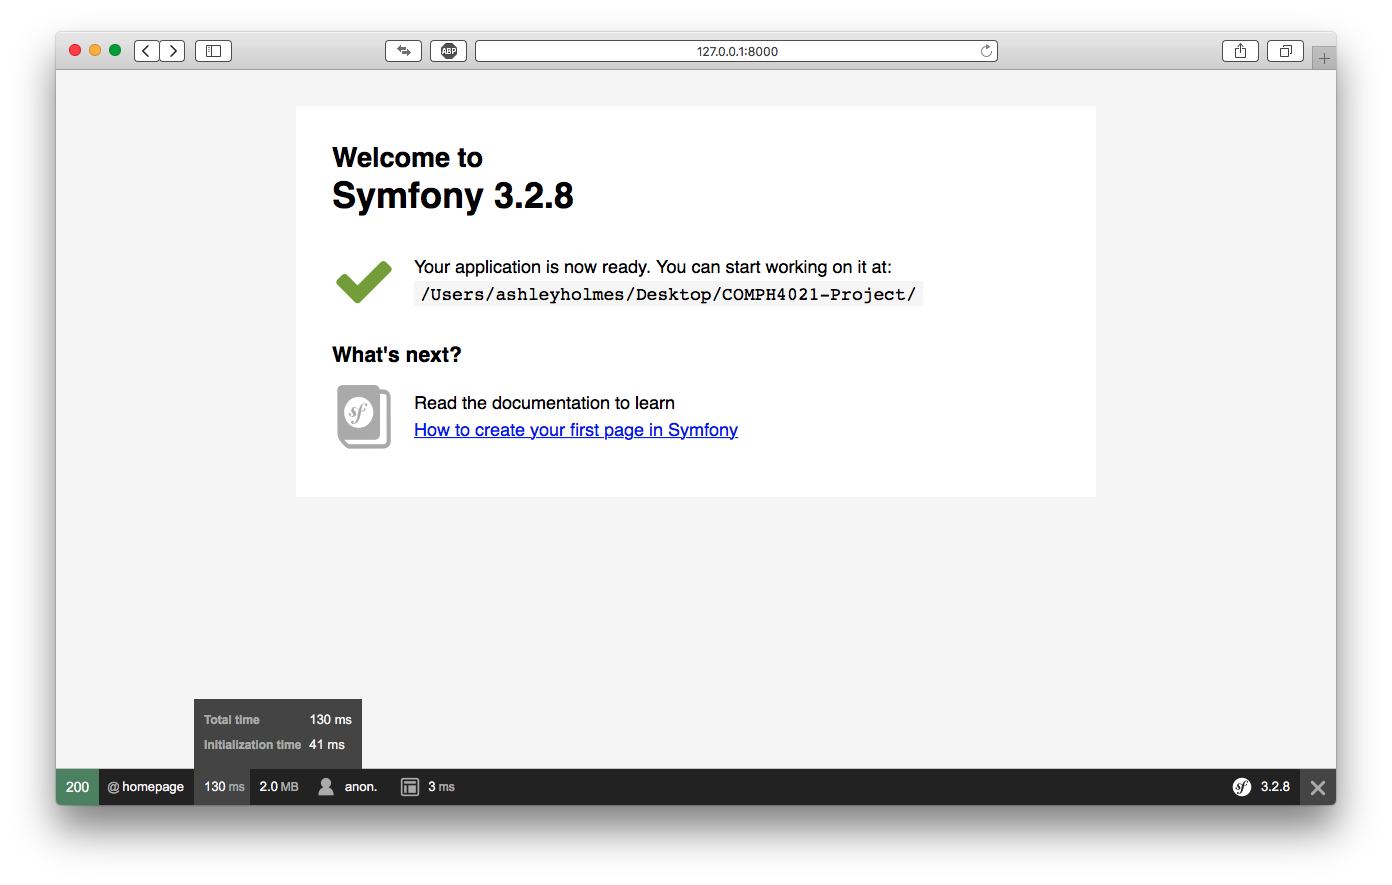
\includegraphics[width=400pt]{figures/webdebug_2.png} % requires the graphicx package
   \caption{Web Debug Toolbar and Profiler Extended}
   \label{fig:Web Debug Toolbar and Profiler Extended}
\end{figure}

\begin{figure}[htbp]
   \centering
   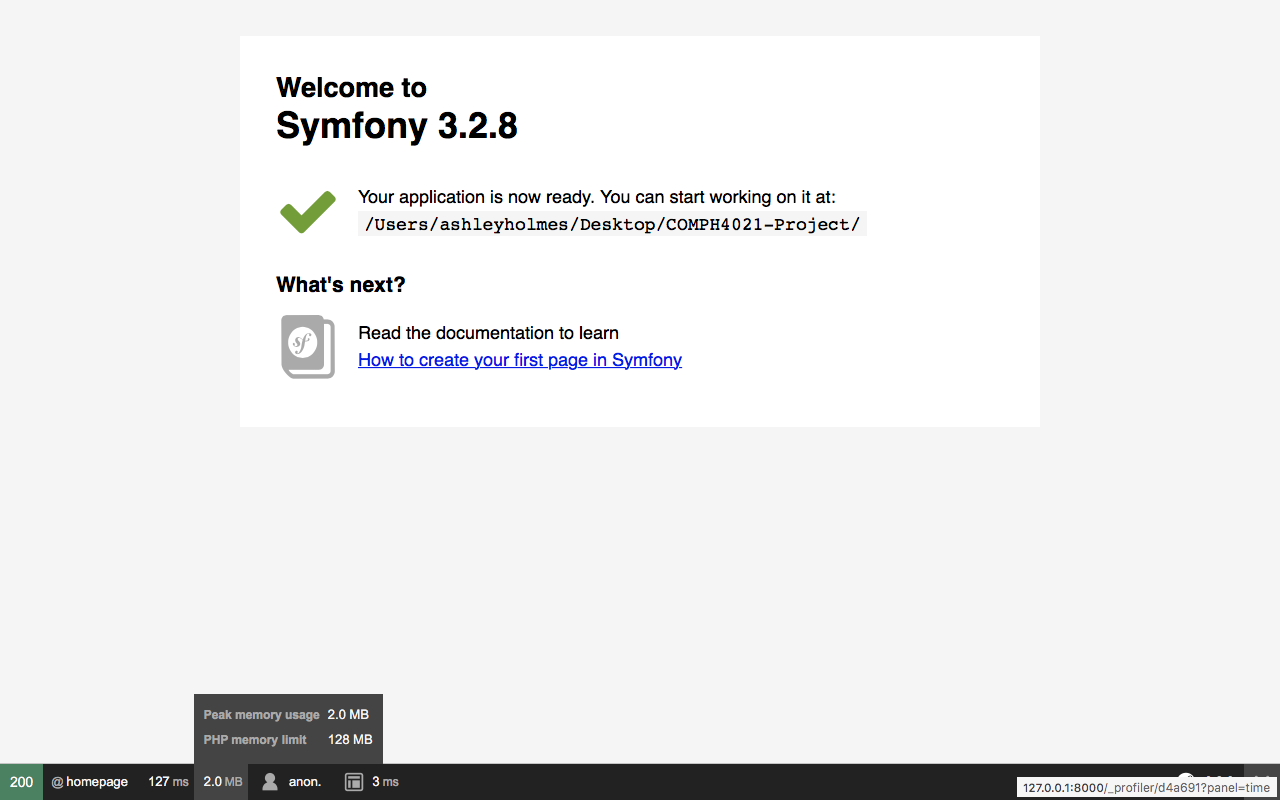
\includegraphics[width=400pt]{figures/webdebug_3.png} % requires the graphicx package
   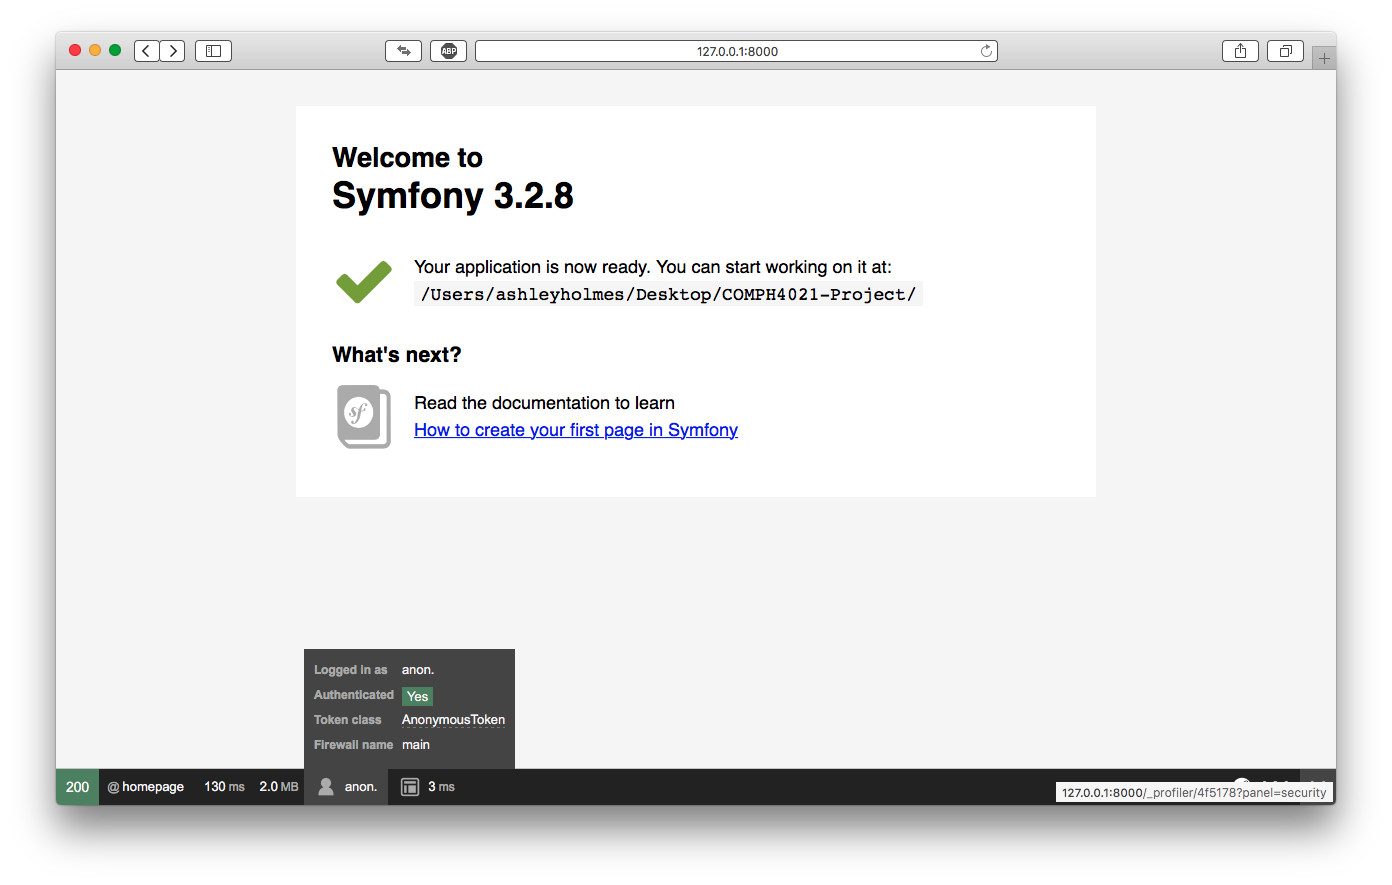
\includegraphics[width=400pt]{figures/webdebug_4.png}
   \caption{Web Debug Toolbar and Profiler Extended}
   \label{fig:Web Debug Toolbar and Profiler Extended}
\end{figure}

\begin{figure}[htbp]
   \centering
   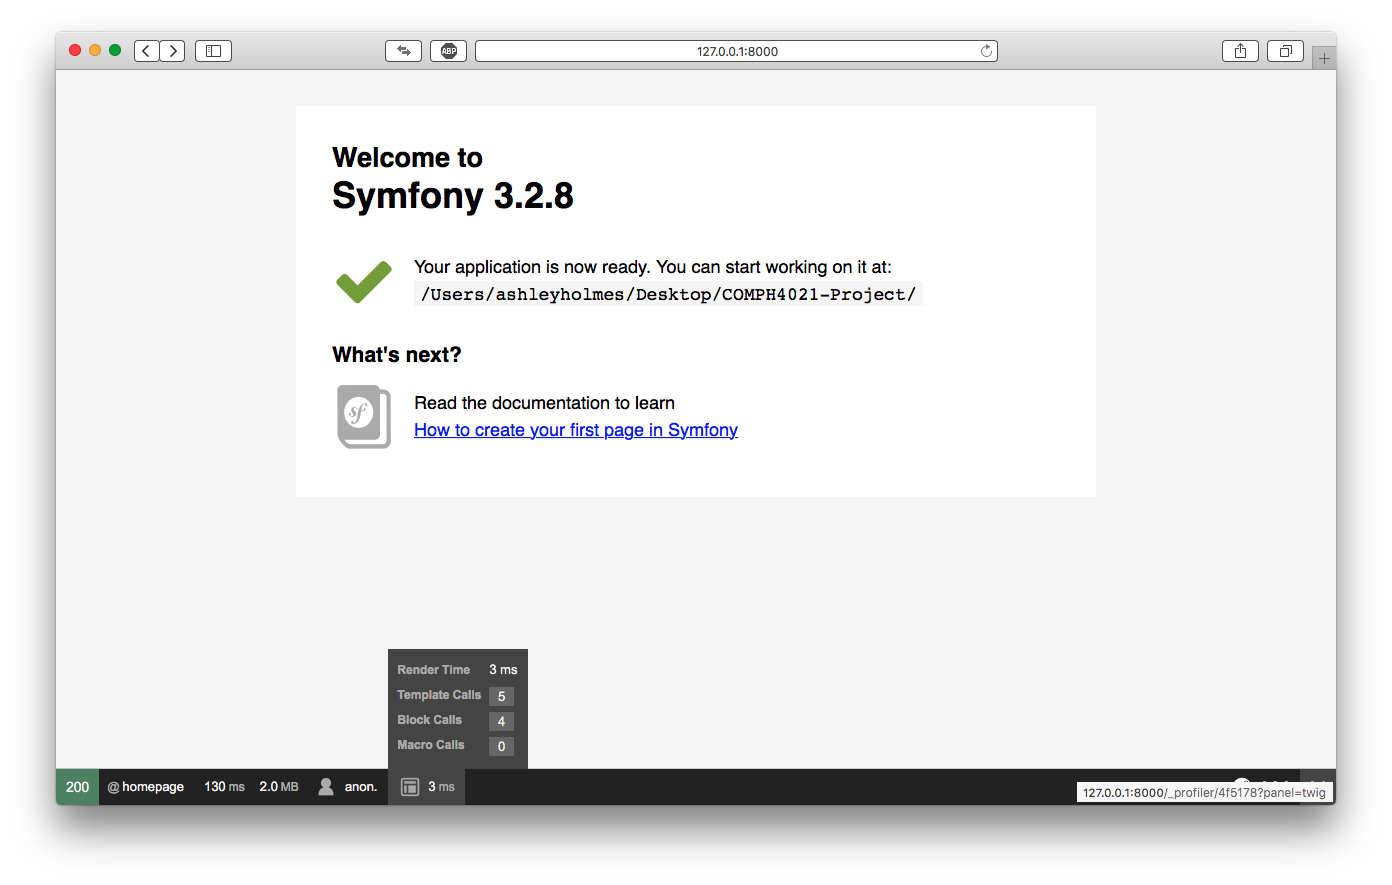
\includegraphics[width=400pt]{figures/webdebug_5.png}
   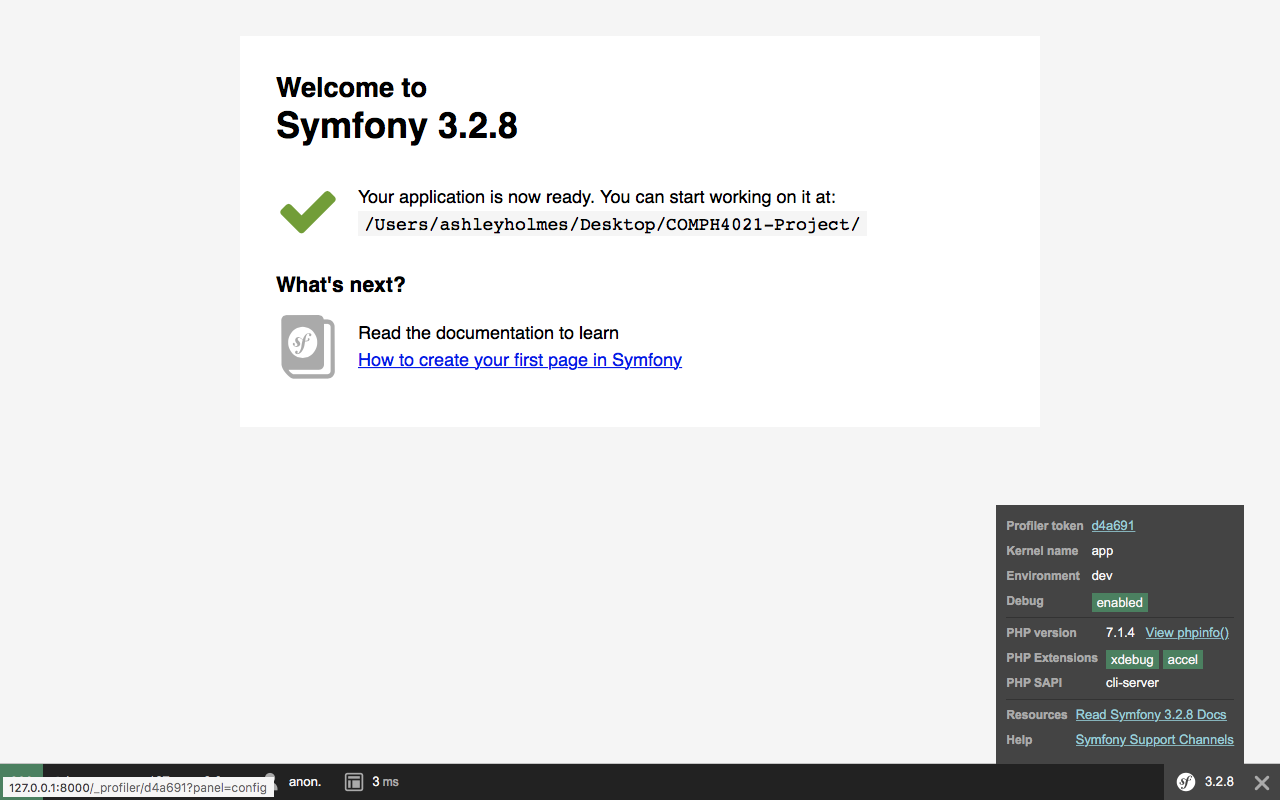
\includegraphics[width=400pt]{figures/webdebug_6.png} % requires the graphicx package
   \caption{Web Debug Toolbar and Profiler Extended}
   \label{fig:Web Debug Toolbar and Profiler Extended}
\end{figure}

Now that the configuration phase has been completed one now navigates to the browser and using the URL http://localhost:8000 as shown in the terminal window in figure \ref{fig:Terminal Window Bottom} under the Run your application heading. This brings up the following page in figure \ref{fig:Symfony Browser}. It is being executed by the Symfony framework from the files inside the project folder. The code is depicted in figure \ref{fig:Web Debug Toolbar and Profiler}. In the bottom of the window is the web debug toolbar which is in a maximised position and can be minimised by clicking on the X in the right hand corner. This often offers better visibility when developing. If the mouse is used to hover over the toolbar it will display information such as routing, controllers which were executed, time it took to load the page, which way the user is authenticated on the page and more debugging information and a link to the resources and documentation as shown in figure \ref{fig:Web Debug Toolbar and Profiler Extended}. Clicking on the icons will give much more information. The URL http://127.0.0.1:8000/config.php would show the user the instructions needed for further configuration. This is reference to figure \ref{fig:Configuration Checker}.


\begin{figure}[htbp]
   \centering
   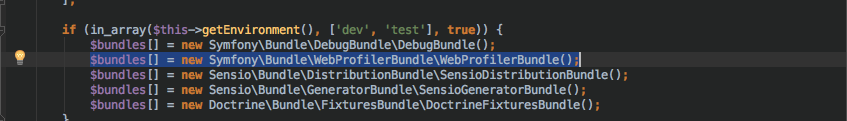
\includegraphics[width=400pt]{figures/AppKernel.png}
   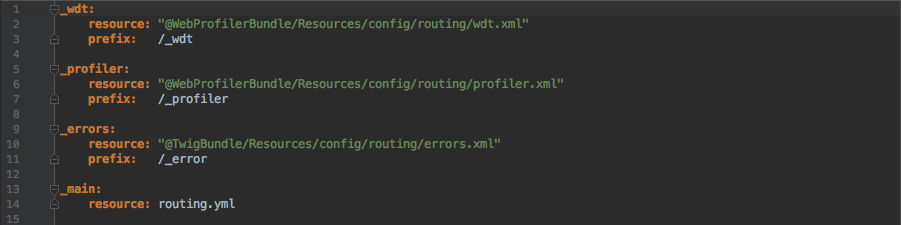
\includegraphics[width=400pt]{figures/routing_dev.png}
   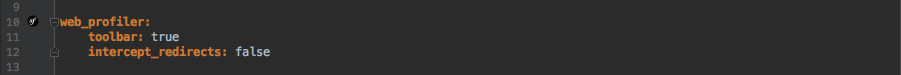
\includegraphics[width=400pt]{figures/config_dev.png} % requires the graphicx package
   \caption{Web Debug Toolbar and Profiler}
   \label{fig:Web Debug Toolbar and Profiler}
\end{figure}

\section{IDE}

\subsection{PhpStorm IDE for PHP}

\begin{figure}[htbp]
   \centering
   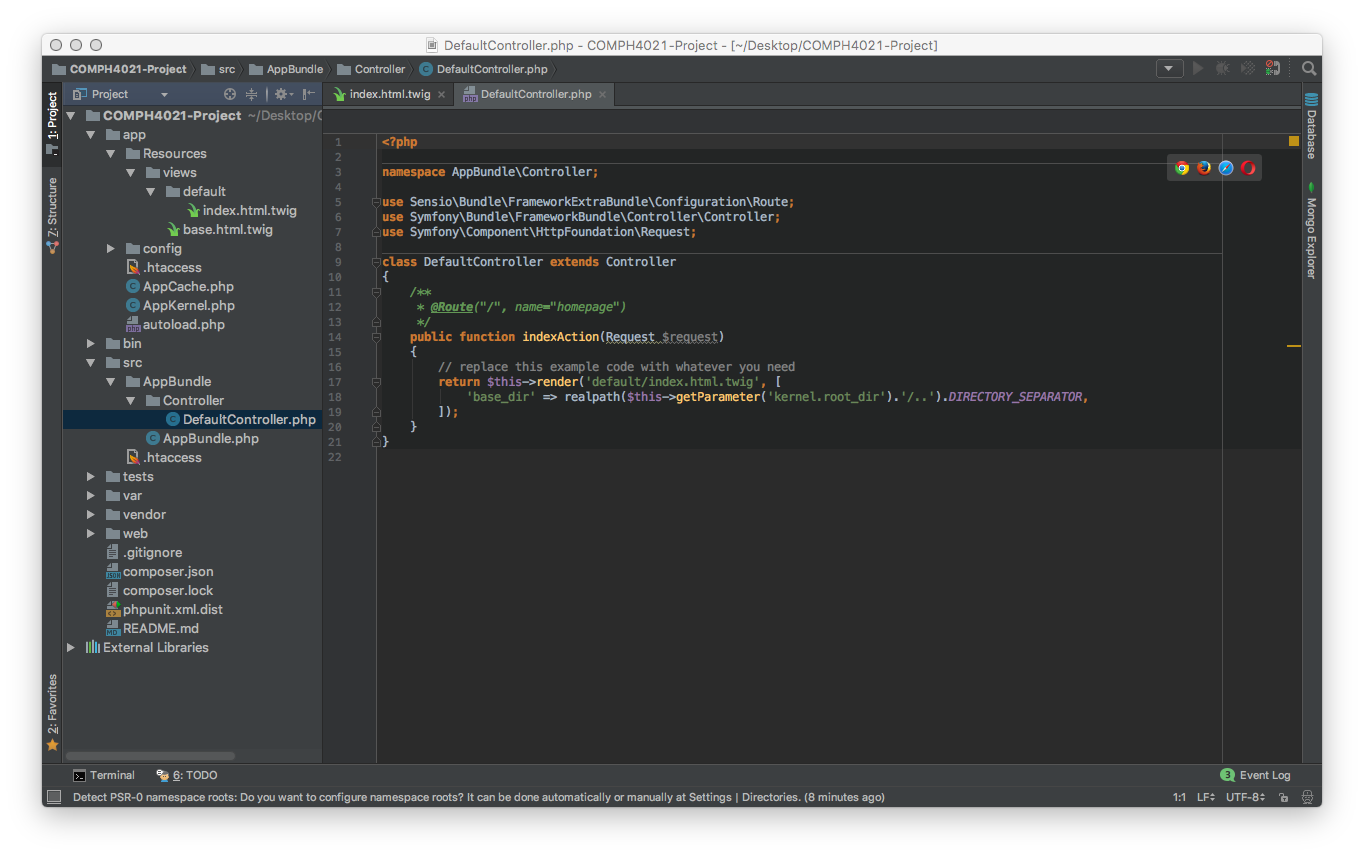
\includegraphics[width=400pt]{figures/default_controller.png} % requires the graphicx package
   \caption{Default Controller}
   \label{fig:Default Controller}
\end{figure}

Most of the files live in src/AppBundle. Looking at the controller called Default Controller in the below figure \ref{fig:Default Controller}. This controller class defines what is seen in figure \ref{fig:Symfony Browser}. It renders the Symfony Welcome Page. Take note of the @Route("/", name="homepage") annotation on line 12. It matches the route in figure \ref{fig:Web Debug Toolbar and Profiler Extended}.













